% ========== Template by IC\M/T Institute of Creative\Media/Technologies =============
% ==========  M. Wagner and K. Blumenstein, 2021 ============= 
% ==========  Based on the LaTeX Thesis Template for the University of Applied Sciences St.Pölten by P. Lechner https://github.com/hrtlacek/ThesisTemplate-FH-StP        ============= 

%----------------------------------------------------------------
% TODO List


%----------------------------------------------------------------

% ============= Settings for the Work =============

%***************************************************************************************

% Place your data here!!!

\def\workTitle{<Title of the Work>}
\def\subTitle{<Subtitle>}
\def\specialization{<Name of Masterclass>}
\def\studentFirstName{<FirstName>}
\def\studentLastName{<LastName>}
\def\studentId{<StudentID>}
\def\advisorPreTitle{<Pre-Title>}
\def\advisoFirstName{<FirstName>}
\def\advisorLastName{<LastName>}
\def\advisorPosTitle{<Pos-Title>}
\def\assessorPreTitle{<Pre-Title>}
\def\assessorFirstName{<FirstName>}
\def\assessorLastName{<LastName>}
\def\assessorPosTitle{<Pos-Title>}
\def\place{<Place>}
\def\dateDay{<DD>}
\def\dateMonth{<MM>}
\def\dateYear{<YYYY>}

%***************************************************************************************

\newif\ifUseOneSide                         % <== DONT TOUCH THIS!!!
\newif\ifUseGermanVersion				    % <== DONT TOUCH THIS!!!
\newif\ifUseMasterInteractiveTechnologies 	% <== CAN'T TOUCH THIS!!! (da da dada)
\newif\ifUseMasterDigitalDesign	            % <== DONT TOUCH THIS!!!
\newif\ifUseMasterDigitalMediaProduction	% <== DONT TOUCH THIS!!!
\newif\ifUseMasterDigitalHealthCare			% <== DONT TOUCH THIS!!!
\newif\ifUseBachelorMediaTechnologies       % <== DONT TOUCH THIS!!!
\newif\ifUseBachelorSmartEngineering        % <== DONT TOUCH THIS!!!
\newif\ifUseBachelorCreativeComputing       % <== DONT TOUCH THIS!!!

%To switch between one or two side layout
\UseOneSidetrue                             % Using the one side layout
%\UseOneSidefalse                            % Using the two side layout
% *** ATTENTION: When using double page layout, you need to print the Title Page as a single Page!!! ***

%***************************************************************************************

% To switch the version please use the comment "%" option :-). After a language change, you have to rebuild the whole project (in Overleaf --> recompile from scratch) 
%\UseGermanVersiontrue					    % German version
\UseGermanVersionfalse					    % English version

%***************************************************************************************

% To switch between the study programs use the comment option :-) 
% !!!ATTENTION: Only one has to be activated!!!

%\UseBachelorMediaTechnologiestrue		   % Bachelor Media Technology
\UseBachelorSmartEngineeringtrue		    % Bachelor Smart Engineering
%\UseBachelorCreativeComputingtrue		    % Bachelor Creative Computing
%\UseMasterInteractiveTechnologiestrue		% Master Interactive Technologies
%\UseMasterDigitalDesigntrue		        % Master Digital Design
%\UseMasterDigitalMediaProductiontrue		% Master Digital Media Production
%\UseMasterDigitalHealthCaretrue			% Master Digital Health Care

%***************************************************************************************
%Dokumentklasse without end dot ;-)
%\documentclass[a4paper,twoside,11pt, numbers=noenddot]{scrreprt
%\PassOptionsToPackage[english,ngerman]{babel}
\ifUseOneSide
    \documentclass[a4paper,oneside,11pt, numbers=noenddot]{scrreprt}%{book}{report}
\else
    \documentclass[a4paper,twoside,11pt, numbers=noenddot]{scrreprt}%{book}{report}
\fi
\usepackage[ngerman, english]{babel}
\usepackage[left= 3.5cm,right = 3cm, bottom = 3.5 cm, top = 3 cm]{geometry}
\usepackage[onehalfspacing]{setspace}

% Standard Packages
\usepackage[utf8]{inputenc}

% ============= Packages =============

% Document information
\usepackage[
	pdftitle={\workTitle},
	pdfsubject={},
	pdfauthor={\studentFirstName \studentLastName},
	pdfkeywords={}
	pdftex=true, 
	colorlinks=true,
 	breaklinks=true,
	citecolor=black,
	linkcolor=black,	
	menucolor=black,	
	urlcolor=black
]{hyperref}

\hypersetup{
    %bookmarks=true,         % show bookmarks bar?
    unicode=false,          % non-Latin characters in Acrobat’s bookmarks
    pdftoolbar=true,        % show Acrobat’s toolbar?
    pdfmenubar=true,        % show Acrobat’s menu?
    pdffitwindow=false,     % window fit to page when opened
    pdfstartview={FitH},    % fits the width of the page to the window
    pdftitle={My title},    % title
    pdfauthor={Author},     % author
    pdfsubject={Subject},   % subject of the document
    pdfcreator={Creator},   % creator of the document
    pdfproducer={Producer}, % producer of the document
    pdfkeywords={keyword1} {key2} {key3}, % list of keywords
    pdfnewwindow=true,      % links in new window
    colorlinks=false,       % false: boxed links; true: colored links
    linkcolor=black,          % color of internal links (change box color with linkbordercolor)
    citecolor=black,        % color of links to bibliography
    filecolor=black,      % color of file links
    urlcolor=black           % color of external links
}

\usepackage{csquotes}

\usepackage[T1]{fontenc}
\usepackage{graphicx, subfigure}
\usepackage{fancyhdr}
\usepackage{lmodern}
\usepackage{color}
\usepackage{transparent}

\usepackage[backend=biber, style=apa, citestyle=authoryear, sorting=nyt]{biblatex}
% Usable sorting styles are:
% nty = Sort by name, title, year.
% nyt = Sort by name, year, title.
% nyvt = Sort by name, year, volume, title.
% anyt = Sort by alphabetic label, name, year, title.
% anyvt = Sort by alphabetic label, name, year, volume, title.
% ynt = Sort by year, name, title.
% ydnt = Sort by year (descending), name, title.
% none = Do not sort at all. All entries are processed in citation order.
% debug = Sort by entry key. This is intended for debugging only.

% Switch the language
\ifUseGermanVersion
    \DeclareLanguageMapping{ngerman}{ngerman-apa}
\else
    \DeclareLanguageMapping{english}{english-apa}
\fi

\addbibresource{biblatex.bib}

% Additional letters from the American Mathematical Society
\usepackage{amsfonts}
\usepackage{mathtools}

\usepackage[export]{adjustbox}

% Block Diagram Drawing Package
% ---tikz
\usepackage{tikz}
\usetikzlibrary{positioning}
\usepackage{pgfplots}
\pgfplotsset{compat=1.10}
\usepackage{textcomp}

%Package for using the [H] option on graphics to force them into place
\usepackage{float}

%iPython packages:
%\usepackage{graphicx} % Used to insert images
\usepackage{adjustbox} % Used to constrain images to a maximum size 
\usepackage{color} % Allow colors to be defined
\usepackage{enumerate} % Needed for markdown enumerations to work
\usepackage{geometry} % Used to adjust the document margins
\usepackage{amsmath} % Equations
\usepackage{amssymb} % Equations
%\usepackage[mathletters]{ucs} % Extended unicode (utf-8) support
% \usepackage[utf8x]{inputenc} % Allow utf-8 characters in the tex document
\usepackage{fancyvrb} % verbatim replacement that allows latex
\usepackage{grffile} % extends the file name processing of package graphics 
                         % to support a larger range 
    % The hyperref package gives us a pdf with properly built
    % internal navigation ('pdf bookmarks' for the table of contents,
    % internal cross-reference links, web links for URLs, etc.)
\usepackage{hyperref}
\usepackage{longtable} % longtable support required by pandoc >1.10

% embedding of audio/video files etc.
% \usepackage{attachfile}
% \usepackage{movie15}
% \usepackage{media9}
% \usepackage{menukeys}

\usepackage[labelfont=it, labelsep=period, format=plain,justification=raggedright, singlelinecheck=false]{caption}
\captionsetup[figure]{justification=centering}
\definecolor{light-gray}{gray}{0.85}

% Switch between German and English based on the Settingx.tex. file
\usepackage{ifthen}

% =============== Block Diagram Drawing Config
\usetikzlibrary{shapes,arrows}

% Definition of blocks:
\tikzset{%
  block/.style    = {draw, thick, rectangle, minimum height = 3em,
    minimum width = 3em},
  sum/.style      = {draw, circle, node distance = 2cm}, % Adder
  input/.style    = {coordinate}, % Input
  output/.style   = {coordinate}, % Output
  mult/.style	  = {draw, isosceles triangle, minimum height=1cm, minimum width =1cm}
}
%mult/.style	  = {isosceles triangle, sharp corners, anchor=center, xshift=-4mm, minimum height=1.5cm, minimum width =0.05cm}
%isosceles triangle, fill=gray!25, minimum width=1.5cm

% Defining string as labels of certain blocks.
\newcommand{\suma}{\Large$+$}
\newcommand{\inte}{$\displaystyle \int$}
\newcommand{\derv}{\huge$\frac{d}{dt}$}
\newcommand{\conv}{\huge$\ast$}

% ============================================

% -- Settings für Code abbildungen
\usepackage{listings,lstautogobble}
\lstset{backgroundcolor=\color{light-gray},frame=single, framerule=0pt, showspaces=false, showtabs=false, numbers=left, numbersep=5pt, breaklines=false, autogobble=true, language=C++}

% Setze arial font
\usepackage[scaled]{helvet}
\renewcommand*{\familydefault}{\sfdefault}

% FH-green blue
\definecolor{FH}{rgb}{0.10, 0.57, 0.68}
% FH-green blue 2
\definecolor{FH2}{rgb}{0.0392, 0.666, 0.549}

% No indention afer a paragraph
\setlength{\parindent}{0cm}

% Paragraph
\setlength{\parskip}{0.3cm}

% ============= Header and Footer =============

\renewcommand{\chaptermark}[1]{\markboth{\thechapter~ #1}{}}

\ifUseOneSide
\fancypagestyle{icmt}{%
  \fancyhf{}% Clear header and footer
  \fancyhead[L]{\leftmark}
  \fancyfoot[R]{\thepage}% Custom footer
  \renewcommand{\headrulewidth}{0.4pt}% Line at the header visible
  \renewcommand{\footrulewidth}{0.0pt}% Line at the footer visible
}
% Redefine the plain page style
\fancypagestyle{plain}{%
  \fancyhf{}%
  \fancyfoot[R]{\thepage}%
  \renewcommand{\headrulewidth}{0.0pt}% Line at the header invisible
  \renewcommand{\footrulewidth}{0.0pt}% Line at the footer visible
}
\else
\fancypagestyle{icmt}{%
  \fancyhf{}% Clear header and footer
  \fancyhead[L]{\leftmark}
  \fancyfoot[RO,LE]{\thepage}% Custom footer
  \renewcommand{\headrulewidth}{0.4pt}% Line at the header visible
  \renewcommand{\footrulewidth}{0.0pt}% Line at the footer visible
}
% Redefine the plain page style
\fancypagestyle{plain}{%
  \fancyhf{}%
  \fancyfoot[RO,LE]{\thepage}%
  \renewcommand{\headrulewidth}{0.0pt}% Line at the header invisible
  \renewcommand{\footrulewidth}{0.0pt}% Line at the footer visible
  }
\fi

% ============= Package Settings & Others ============= 


% Special Spellings
\hyphenation{De-zi-mal-tren-nung St-rei-fen-licht-scan-nern}

% Roman itemization \RM{<Number>}
\newcommand{\RM}[1]{\MakeUppercase{\romannumeral #1}}


% ============= Dokumentbeginn =============

\begin{document}
\ifUseGermanVersion
	\selectlanguage{ngerman}
\else
	\selectlanguage{english}
\fi

% Select the right main page ;-)
\ifUseGermanVersion
	
% setup page dimensions for titlepage
\newgeometry{left=2.4cm,right=2.4cm,bottom=2.5cm,top=2cm}


% first titlepage
\pagestyle{empty}

\begin{figure}[H]
\vspace*{-2.5cm}
\hspace*{2.5cm}

\includegraphics[keepaspectratio, width=1.4\textwidth, right]{TemplateElements/fhLogo3.png}
\end{figure}


\begin{center}

\vspace{1cm}

\begin{minipage}[t][5cm][s]{\textwidth}%
\centering
\Huge{{\color{FH2}{\fontsize{24}{30} \selectfont \workTitle\\}}}
\vspace{0.5cm}
\LARGE{{\color{FH2}{\fontsize{16}{24} \selectfont \subTitle\\}}}
\end{minipage}

\vspace{1cm}


\ifUseBachelorMediaTechnologies
	\LARGE{Bachelorarbeit}
\else
	\ifUseBachelorSmartEngineering
		\LARGE{Bachelorarbeit}
\else
	\ifUseBachelorCreativeComputing
		\LARGE{Bachelorarbeit}
\else
	\ifUseMasterInteractiveTechnologies
		\LARGE{Masterarbeit}
\else
	\ifUseMasterDigitalDesign
		\LARGE{Masterarbeit}
\else
    \ifUseMasterDigitalMediaProduction
		\LARGE{Masterarbeit}
\else
	\ifUseMasterDigitalHealthCare
		\LARGE{Masterarbeit}
    \else
        \LARGE{YOU HAVE TO CHOOSE THE PROGRAM TYPE IN THE SETTINGS!!!}
  	\fi
\fi
\fi
\fi\fi\fi\fi
  
\vspace{1.3cm}
\ifUseBachelorMediaTechnologies
		\fontsize{11pt}{15pt}\selectfont Bachelor-Studiengang Medientechnik\\
Fachhochschule St. Pölten\\  
\else
	\ifUseBachelorSmartEngineering
    	\fontsize{11pt}{15pt}\selectfont Bachelor-Studiengang Smart Engineering\\
Fachhochschule St. Pölten\\ 
\else
    \ifUseBachelorCreativeComputing
    	\fontsize{11pt}{15pt}\selectfont Bachelor-Studiengang Creative Computing\\
Fachhochschule St. Pölten\\ 
\else
	\ifUseMasterInteractiveTechnologies
		\fontsize{11pt}{15pt}\selectfont Ausgeführt zum Zweck der Erlangung des akademischen Grades\\
		\textbf{Dipl.-Ing. für technisch-wissenschaftliche Berufe}
\else
	\ifUseMasterDigitalDesign
		\fontsize{11pt}{15pt}\selectfont Ausgeführt zum Zweck der Erlangung des akademischen Grades\\
		\textbf{Dipl.-Ing. für technisch-wissenschaftliche Berufe}	
\else
    \ifUseMasterDigitalMediaProduction
		\fontsize{11pt}{15pt}\selectfont Ausgeführt zum Zweck der Erlangung des akademischen Grades\\
		\textbf{Dipl.-Ing. für technisch-wissenschaftliche Berufe}	
\else
	\ifUseMasterDigitalHealthCare
    	\fontsize{11pt}{15pt}\selectfont Ausgeführt zum Zweck der Erlangung des akademischen Grades\\
		\textbf{Master of Science in Engineering (MSc)}
    \else
        \LARGE{YOU HAVE TO CHOOSE THE PROGRAM TYPE IN THE SETTINGS!!!}
\fi\fi\fi\fi\fi\fi\fi

\vspace{4mm}
 
\ifUseMasterInteractiveTechnologies
	am Masterstudiengang Interactive Technologies an der\\ 
Fachhochschule St. Pölten, Masterklasse \specialization
\else
    \ifUseMasterDigitalDesign
	am Masterstudiengang Digital Design an der\\ 
Fachhochschule St. Pölten, Masterklasse \specialization
\else
    \ifUseMasterDigitalMediaProduction
	am Masterstudiengang Digital Media Production an der\\ 
Fachhochschule St. Pölten, Masterklasse \specialization
\else
	\ifUseMasterDigitalHealthCare
		am Masterstudiengang Digital Healthcare\\ 
an der Fachhochschule St. Pölten
    \else
        
\fi\fi\fi\fi

\vspace{1cm}

Ausgeführt von:\\ 
\fontsize{15pt}{15pt}\selectfont
\textbf{\studentFirstName\ \studentLastName} \\
\fontsize{11pt}{15pt}\selectfont
\studentId

\vspace{1cm}
\ifUseBachelorMediaTechnologies
		\begin{tabular}{lll}
        Betreuer/in: & & \advisorPreTitle\ \advisoFirstName\ \advisorLastName, \advisorPosTitle\\
        %Zweitbegutachter/in: & & [Titel Vorname Zuname]
		\end{tabular}
\else
	\ifUseBachelorSmartEngineering
		\begin{tabular}{lll}
        Betreuer/in: & & \advisorPreTitle\ \advisoFirstName\ \advisorLastName, \advisorPosTitle\\
        %Zweitbegutachter/in: & & [Titel Vorname Zuname]
		\end{tabular}
\else
	\ifUseBachelorCreativeComputing
		\begin{tabular}{lll}
        Betreuer/in: & & \advisorPreTitle\ \advisoFirstName\ \advisorLastName, \advisorPosTitle\\
        %Zweitbegutachter/in: & & [Titel Vorname Zuname]
		\end{tabular}
\else
\begin{tabular}{lll}
Betreuer/in: & \advisorPreTitle\ \advisoFirstName\ \advisorLastName, \advisorPosTitle\\
Zweitbetreuer/in: & \assessorPreTitle\ \assessorFirstName\ \assessorLastName, \assessorPosTitle\\
\end{tabular}

\fi
\fi
\fi

\vspace{1cm}


\large{\place, \dateDay.\dateMonth.\dateYear}


\end{center}

\restoregeometry
\else
	
% setup page dimensions for titlepage
\newgeometry{left=2.4cm,right=2.4cm,bottom=2.5cm,top=2cm}


% first titlepage
\pagestyle{empty}

\begin{figure}[H]
\vspace*{-2.5cm}
\hspace*{2.5cm}

\includegraphics[keepaspectratio, width=1.4\textwidth, right]{TemplateElements/fhLogo3.png}
\end{figure}



\begin{center}

\vspace{1cm}

\begin{minipage}[t][5cm][s]{\textwidth}%
\centering
\Huge{{\color{FH2}{\fontsize{24}{30} \selectfont \workTitle\\}}}
\vspace{0.5cm}
\LARGE{{\color{FH2}{\fontsize{16}{24} \selectfont \subTitle\\}}}
\end{minipage}

\vspace{1cm}


\ifUseBachelorMediaTechnologies
	\LARGE{Bachelor Thesis}
\else
	\ifUseBachelorSmartEngineering
		\LARGE{Bachelor Thesis}
\else
	\ifUseBachelorCreativeComputing
		\LARGE{Bachelor Thesis}
\else
	\ifUseMasterInteractiveTechnologies
		\LARGE{Master Thesis}
\else
	\ifUseMasterDigitalDesign
		\LARGE{Master Thesis}
\else
    \ifUseMasterDigitalMediaProduction
		\LARGE{Master Thesis}
\else
	\ifUseMasterDigitalHealthCare
		\LARGE{Master Thesis}
    \else
        \LARGE{YOU HAVE TO CHOOSE THE PROGRAM TYPE IN THE SETTINGS!!!}
  	\fi
\fi
\fi
\fi\fi\fi\fi
  
\vspace{1.3cm}
\ifUseBachelorMediaTechnologies
		\fontsize{11pt}{15pt}\selectfont Bachelor Course on Media Technology\\
at St. Pölten University of Applied Sciences\\  
\else
	\ifUseBachelorSmartEngineering
		\fontsize{11pt}{15pt}\selectfont Bachelor Course on Smart Engineering\\
at St. Pölten University of Applied Sciences\\  
\else
	\ifUseBachelorCreativeComputing
		\fontsize{11pt}{15pt}\selectfont Bachelor Course on Creative Computing\\
at St. Pölten University of Applied Sciences\\  
\else
	\ifUseMasterInteractiveTechnologies
		\fontsize{11pt}{15pt}\selectfont For attainment of the academic degree of\\
		\textbf{Dipl.-Ing. für technisch-wissenschaftliche Berufe}
\else
    \ifUseMasterDigitalDesign
		\fontsize{11pt}{15pt}\selectfont For attainment of the academic degree of\\
		\textbf{Dipl.-Ing. für technisch-wissenschaftliche Berufe}
\else
    \ifUseMasterDigitalMediaProduction
		\fontsize{11pt}{15pt}\selectfont For attainment of the academic degree of\\
		\textbf{Dipl.-Ing. für technisch-wissenschaftliche Berufe}
\else
	\ifUseMasterDigitalHealthCare
    	\fontsize{11pt}{15pt}\selectfont For attainment of the academic degree of\\
		\textbf{Master of Science in Engineering (MSc)}
    \else
        \LARGE{YOU HAVE TO CHOOSE THE PROGRAM TYPE IN THE SETTINGS!!!}
  	\fi
\fi
\fi
\fi\fi\fi
\fi

\vspace{4mm}
 
\ifUseMasterInteractiveTechnologies
	in the Masters Course Interactive Technologies at St. Pölten\\ 
University of Applied Sciences, Masterclass \specialization
\else
    \ifUseMasterDigitalDesign
	in the Masters Course Digital Design at St. Pölten\\ 
University of Applied Sciences, Masterclass \specialization
\else
    \ifUseMasterDigitalMediaProduction
	in the Masters Course Digital Media Production at St. Pölten\\ 
University of Applied Sciences, Masterclass \specialization
\else
	\ifUseMasterDigitalHealthCare
		in the Masters Course Digital Healthcare\\ 
at St. Pölten University of Applied Sciences
    \else
  	\fi
\fi\fi\fi





\vspace{1cm}

Submitted by:\\ 
\fontsize{15pt}{15pt}\selectfont
\textbf{\studentFirstName\ \studentLastName} \\
\fontsize{11pt}{15pt}\selectfont
\studentId

\vspace{1cm}
\ifUseBachelorMediaTechnologies
		\begin{tabular}{lll}
        Advisor: & & \advisorPreTitle\ \advisoFirstName\ \advisorLastName, \advisorPosTitle\\
        %Zweitbegutachter/in: & & [Titel Vorname Zuname]
		\end{tabular}
\else
	\ifUseBachelorSmartEngineering
		\begin{tabular}{lll}
        Advisor: & & \advisorPreTitle\ \advisoFirstName\ \advisorLastName, \advisorPosTitle\\
        %Zweitbegutachter/in: & & [Titel Vorname Zuname]
		\end{tabular}
\else
	\ifUseBachelorCreativeComputing
		\begin{tabular}{lll}
        Advisor: & & \advisorPreTitle\ \advisoFirstName\ \advisorLastName, \advisorPosTitle\\
        %Zweitbegutachter/in: & & [Titel Vorname Zuname]
		\end{tabular}
\else
  \begin{tabular}{lll}
  Advisor: & \advisorPreTitle\ \advisoFirstName\ \advisorLastName, \advisorPosTitle\\
  Second Advisor: & \assessorPreTitle\ \assessorFirstName\ \assessorLastName, \assessorPosTitle\\
  \end{tabular}

\fi
\fi
\fi

\vspace{1cm}


\large{\place, \dateDay.\dateMonth.\dateYear}


\end{center}

\restoregeometry
\fi

% \part No numbering in the table of contend
\makeatletter
\let\partbackup\l@part
\renewcommand*\l@part[2]{\partbackup{#1}{}}

% Restart of the page numbering, Numbers [arabic], Roman numbers [roman,Roman], letters [alph,Alph]
\pagenumbering{Roman}
   
\pagestyle{plain}
\ifUseGermanVersion
	\chapter*{Ehrenwörtliche Erklärung}
\label{ch:erklaerung}

\begin{flushleft}
Ich versichere, dass 
\end{flushleft}

\begin{flushleft}
- ich diese Arbeit selbständig verfasst, andere als die angegebenen Quellen und Hilfsmittel nicht benutzt und mich sonst keiner unerlaubten Hilfe bedient habe.
\end{flushleft}

\begin{flushleft}
- ich dieses Thema bisher weder im Inland noch im Ausland einem Begutachter/ einer Begutachterin zur Beurteilung oder in irgendeiner Form als Prüfungsarbeit vorgelegt habe.	
\end{flushleft}

\begin{flushleft}
- diese Arbeit mit der vom Begutachter/von der Begutachterin beurteilten Arbeit übereinstimmt. \\[1.5cm]	
\end{flushleft}
% - diese Arbeit mit der vom Begutachter/von der Begutachterin beurteilten Arbeit übereinstimmt. \\
% \\[1.5cm]
Datum:	\hrulefill\enspace Unterschrift: \hrulefill
\\[3.5cm]
\else
	\chapter*{Declaration}
\label{ch:declaration}

\begin{flushleft}
I assure that 
\end{flushleft}

\begin{flushleft}
- I have written this work independently, have not used other sources and aids than those indicated and have not made use of any other unauthorized assistance.
\end{flushleft}

\begin{flushleft}
- I have not yet submitted this topic to an assessor in Austria or abroad for assessment or in any form as an examination paper.
\end{flushleft}

\begin{flushleft}
- this work corresponds to the work assessed by the assessor.
\end{flushleft}

\vspace{1.5cm}

Date:	\hrulefill\enspace Signature: \hrulefill
\\[3.5cm]
\fi

\newpage
%\chapter*{Kurzfassung}
%\label{ch:kurzfassung}
%Dies ist die Kurzfassung der Arbeit. Lorem ipsum dolor sit amet, consectetur adipisicing elit, sed do eiusmod
%tempor incididunt ut labore et dolore magna aliqua. Ut enim ad minim veniam,
%quis nostrud exercitation ullamco laboris nisi ut aliquip ex ea commodo
%consequat. Duis aute irure dolor in reprehenderit in voluptate velit esse
%cillum dolore eu fugiat nulla pariatur. Excepteur sint occaecat cupidatat non
%proident, sunt in culpa qui officia deserunt mollit anim id est laborum.


%\newpage

\chapter*{Abstract}
\label{ch:abstract}

Introduction: Warum behandeln wir das Thema

Purpose: Welches Problem soll gelöst werden

Method: Wie wurde die Problemlösung gemacht

Product: Was war das Ergebnis

Conclusion: Was sind die Folgerungen / Schlussfolgerungen aus den gewonnen Erkenntnissen

keine Referenzen und Zitate


\chapter*{Kurzfassung}
\label{ch:kurzfassung}

Das Abstract auf deutsch.

\newpage

% Table of Contend
\tableofcontents

\newpage
% Restart of the page numbering, Numbers [arabic], Roman numbers [roman,Roman], letters [alph,Alph]
\pagenumbering{arabic}

% Activate page style for the whole document
\pagestyle{icmt}
\newpage

% /*================================
% =            EXAMPLE            =
% ================================*/

% Delete this include at the end
\chapter{Example}
\label{ch:example}

!!! Please delete this chapter after finishing your work !!!

\section{Settings}

To add your name and the title of your work, please use the ``Settings.tex'' file!
Additionally, switch there between German and English version.

\section{How to Make Sections and Subsections}

Use section and subsection commands to organize your document. \LaTeX{} handles all the formatting and numbering automatically. Use ref and label commands for cross-references.

\subsection{How to Make Lists}

You can make lists with automatic numbering \dots

\begin{enumerate}
\item Like this,
\item and like this.
\end{enumerate}
\dots or bullet points \dots
\begin{itemize}
\item Like this,
\item and like this.
\end{itemize}
\dots or with words and descriptions \dots
\begin{description}
\item[Word] Definition
\item[Concept] Explanation
\item[Idea] Text
\end{description}

\section{Section}

You have to write text between each headline.

\section{Citation}

This part describes the three types of citations which are possible:

\section{Direct Citation}

The maximum for a direct citation is a ${1/2}$ page.

\begin{quotation}
	Overview first, zoom and filter, then details-on-demand
	\autocite{shneiderman_eyes_1996}
\end{quotation}

\section{Floating Text Citation}

\textcite{shneiderman_eyes_1996} defined the Visual Information Seeking Mantra as ``Overview first, zoom and filter, then details-on-demand''.

\section{Indirect Citation}

Some text which summarizes a paper or a book chapter. This could take several lines.
Find attached a citation of a website~\autocite{kaley_match_2018}.

\newpage
\section{Figures}

To place a figure use the following code example

\begin{figure}[ht!]
  \centering
  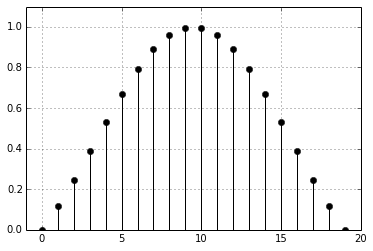
\includegraphics[width=1\columnwidth]{Figures/Example}
  \caption{Interactive data exploration with multiple devices.}
  \label{fig:example}
\end{figure}

$$\int{a,b}$$


\begin{figure}[h]
    \centering
    \subfigure[Figure A]{
    	\label{fig:a}
        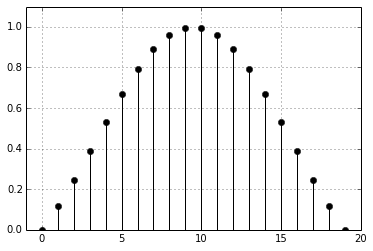
\includegraphics[width=60mm]{Figures/Example}
     }
	\subfigure[Figure B]{
    	\label{fig:b}
        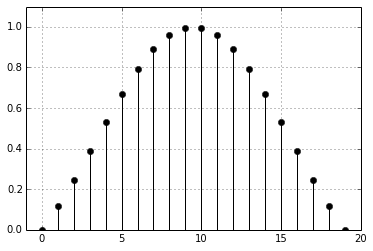
\includegraphics[width=60mm]{Figures/Example}
     }
    \caption{Wearables worn for experiments 1, 2, and 3.}\label{fig:figure2}
\end{figure}

Refer to a figure in the following forms:\\
If you take a look at Figure~\ref{fig:example} ...\\
... text text (see Figure~\ref{fig:example}) ...

\section{Listings}
\begin{lstlisting}[caption=A bit of source code., label=lst:test]
if( true == questions )
{
    std::cout << "Let me google it for you";
}
else
{
    std::cout << "Great";
}
\end{lstlisting}

Now lets take a look at Listing~\ref{lst:test}.


\section{Table}

\begin{table}[ht!]
  \caption{My caption with a very useful description. die kann auch etwas länger sein und über mehrere Zeilen gehen und so weiter.}
  \label{my-label}
  \begin{tabular}{llr}
    \hline
    \multicolumn{2}{c}{Item} &            \\ \cline{1-2}
    Animal     & Description & Price (\$) \\ \hline
    Gnat       & per gram    & 13.65      \\
               & each        & 0.01       \\
    Gnu        & stuffed     & 92.50      \\
    Emu        & stuffed     & 33.33      \\
    Armadillo  & frozen      & 8.99       \\ \hline
  \end{tabular}
\end{table}

For the fast generation of tables from Excel use \url{http://www.heise.de/download/excel2latex.html}

\section{Equations}

\LaTeX{} is great at typesetting equations. Let $X_1, X_2, \ldots, X_n$ be a sequence of independent and identically distributed random variables with $\text{E}[X_i] = \mu$ and $\text{Var}[X_i] = \sigma^2 < \infty$, and let

$$S_n = \frac{X_1 + X_2 + \cdots + X_n}{n}$$

This was a equation without a label.
      
\begin{equation}
S_n = \frac{1}{n}\sum_{i}^{n} X_i
\label{eq:test}
\end{equation}

This is the reference to equation~\ref{eq:test}.      

denote their mean. Then as $n$ approaches infinity, the random variables $\sqrt{n}(S_n - \mu)$ converge in distribution to a normal $\mathcal{N}(0, \sigma^2)$.




% /*================================
% =            CONTENTS            =
% ================================*/

\chapter{Introduction}
\label{ch:introduction}

\section*{Related work}
\textcite{eitz2012hdhso} collected a dataset of 20,000 sketches and divided them
into 250 categories of 80 images each. Humans recognized on average 73.1\% of 
these sketches correctly. This dataset is used in my work to train and validate
the classifier to choose which animation is the most appropriate to show.

\textcite{10.1145/3469877.3490565} proposes a pipeline to create rigged and
animated characters from a single image. Their solution aims for a holistic
approach, requiring no user intervention, to assist non-professional users in
creating animated characters.
\chapter{Method / Methode}
\label{ch:method}

\section*{Literature review}
I reviewed previous work, focusing on two areas. I explored already available
methods for creating animations from sketches by performing skeleton
classification and reviewed previous work dealing with the classification of
sketched objects.

\section*{Related work}
\textcite{eitz2012hdhso} collected a dataset of 20,000 sketches and divided them
into 250 categories of 80 images each. Humans recognized on average 73.1\% of 
these sketches correctly. This dataset is used in my work to train and validate
the classifier to choose which animation is the most appropriate to show.

\textcite{10.1145/3469877.3490565} proposes a pipeline to create rigged and
animated characters from a single image. Their solution aims for a holistic
approach, requiring no user intervention, to assist non-professional users in
creating animated characters. The proposed pipeline performs contour extraction
with salient object detection and extrudes a 3D mesh from geometry generated by
applying constrained Delaunay to the contours. Afterwards, a skeleton is
estimated using a mean curve method and an animation is transferred onto the
skeleton ==DESCRIBE HOW HERE MAYBE==. In my work, I want to follow a similar
philosophy of no user interaction and hope to improve the believability of the
animated results by not only classifying the skeleton type but also the subject
class of the input sketch.

\chapter{Results / Ergebnisse}
\label{ch:results}

Presenting found literature in a useful way

\section{First Section}
Ich bin Text, Text, Text\footnote{\url{http://mfg.fhstp.ac.at}}


\subsection{First Subsection}
\chapter{Discussion / Diskussion}
\label{ch:discussion}

Comparison of presented technologies/methods/projects

Kritische Diskussion / Vergleich der Ansätze

Welche Methoden werden zumeist genutzt, warum?

Überblick / Zusammenfassung der gefundenen Literatur in einer sinnvollen Kategorisierung / Charakterisierung

\chapter{Conclusion / Fazit}
\label{ch:conclusion}

Was kann man daraus lernen?

Was fehlt?

Ideen für zukünftige Forschung


\pagestyle{plain} 

% References
\newpage
\addcontentsline{toc}{chapter}{Bibliography}
\printbibliography

\ifUseGermanVersion
    % Figures
    \newpage
    \addcontentsline{toc}{chapter}{Abbildungsverzeichnis}
    \listoffigures
    % Tables
    \newpage
    \addcontentsline{toc}{chapter}{Tabellenverzeichnis}
    \listoftables
    % Listings
    \newpage
    \addcontentsline{toc}{chapter}{Quellcodeverzeichnis}
    \lstlistoflistings
    \newpage
\else
	% Figures
    \newpage
    \addcontentsline{toc}{chapter}{List of Figures}
    \listoffigures
    % Tables
    \newpage
    \addcontentsline{toc}{chapter}{List of Tables}
    \listoftables
    % Listings
    \newpage
    \addcontentsline{toc}{chapter}{List of Listings}
    \lstlistoflistings
    \newpage
\fi

% ============================================

\chapter*{Appendices}
\setcounter{section}{0}

\addcontentsline{toc}{chapter}{Appendices}
\renewcommand{\thesection}{\Alph{section}}

\section{Appendix}
\label{appendix_a}

LoHrem ipsum dolor sit amet, consectetur adipisicing elit, sed do eiusmod
tempor incididunt ut labore et dolore magna aliqua. Ut enim ad minim veniam,
quis nostrud exercitation ullamco laboris nisi ut aliquip ex ea commodo
consequat. Duis aute irure dolor in reprehenderit in voluptate velit esse
cillum dolore eu fugiat nulla pariatur. Excepteur sint occaecat cupidatat non
proident, sunt in culpa qui officia deserunt mollit anim id est laborum.LoHrem ipsum dolor sit amet, consectetur adipisicing elit, sed do eiusmod
tempor incididunt ut labore et dolore magna aliqua. Ut enim ad minim veniam,
quis nostrud exercitation ullamco laboris nisi ut aliquip ex ea commodo
consequat. Duis aute irure dolor in reprehenderit in voluptate velit esse
cillum dolore eu fugiat nulla pariatur. Excepteur sint occaecat cupidatat non
proident, sunt in culpa qui officia deserunt mollit anim id est laborum.
LoHrem

\newpage

\section{Appendix}
\label{appendix_b}

LoHrem ipsum dolor sit amet, consectetur adipisicing elit, sed do eiusmod
tempor incididunt ut labore et dolore magna aliqua. Ut enim ad minim veniam,
quis nostrud exercitation ullamco laboris nisi ut aliquip ex ea commodo
consequat. Duis aute irure dolor in reprehenderit in voluptate velit esse
cillum dolore eu fugiat nulla pariatur. Excepteur sint occaecat cupidatat non
proident, sunt in culpa qui officia deserunt mollit anim id est laborum.LoHrem ipsum dolor sit amet, consectetur adipisicing elit, sed do eiusmod
tempor incididunt ut labore et dolore magna aliqua. Ut enim ad minim veniam,
quis nostrud exercitation ullamco laboris nisi ut aliquip ex ea commodo
consequat. Duis aute irure dolor in reprehenderit in voluptate velit esse
cillum dolore eu fugiat nulla pariatur. Excepteur sint occaecat cupidatat non
proident, sunt in culpa qui officia deserunt mollit anim id est laborum.
LoHrem


% ============================================

\end{document}























